% This example uses the 'minted' package, so you need to run the compiler with 
% the '-shell-escape' option, i.e.
% 	pdflatex -shell-escape example.tex
% Additionally, you must have the 'pygmentize' program installed, which is part of 
% the 'Pygments' package (https://pygments.org/)

\documentclass[aspectratio=1610, english]{beamer} 
% Jeśli chcesz otrzymać prezentację w języku polskim, to, powyżej, zamień „english” na „polish”
\usepackage{babel}
\usepackage{booktabs}
\makeatletter
\@ifclasswith{beamer}{english}{
	% \usepackage{english}
    % \usepackage[english]{babel}
}

\makeatother
\usepackage[utf8]{inputenc}
\usepackage{listings} % We want to put listings
\usepackage{minted}   % We want to put listings

\usepackage{csquotes}
\usepackage{tikz}
\usepackage{pgfplots}
\pgfplotsset{compat=1.18}

\mode<beamer>{ 	% In the 'beamer' mode
	\definecolor{links}{HTML}{2A1B81}
	\hypersetup{
		pdfpagemode=FullScreen,                 % Enable Full screen mode
		colorlinks,
		linkcolor=,
		urlcolor=links
	}
	\usetheme[parttitle=rightfooter]{AGH}       % Show part title in right footer
	%\usetheme[nosidebar]{AGH}                  % Do not show sidebar on non-title slides
	%\usetheme[nosidebar, margins=1em]{AGH}     % Do not show sidebar on non-title slides and set both margins (left / right) to 1em
	%\usetheme[dark]{AGH}                       % Use dark background
	%\usetheme[dark, parttitle=leftfooter]{AGH} % Use dark background and show part title in left footer
}
\mode<handout>{	% In the 'handout' mode
	\hypersetup{pdfpagemode=None}		
	\usepackage{pgfpages}
	\pgfpagesuselayout{4 on 1}[a4paper,border shrink=5mm,landscape]	% Show 4 slides on 1 page
	\pgfpageslogicalpageoptions{1}{border code=\pgfusepath{stroke}}
	\pgfpageslogicalpageoptions{2}{border code=\pgfusepath{stroke}}
	\pgfpageslogicalpageoptions{3}{border code=\pgfusepath{stroke}}
	\pgfpageslogicalpageoptions{4}{border code=\pgfusepath{stroke}}
  	\usetheme{boxes}
  	\addheadbox{structure}{\quad\insertpart\hfill\insertsection\hfill\insertsubsection\qquad}          % Content of header
 	\addfootbox{structure}{\quad\insertshortauthor\hfill\insertframenumber\hfill\insertsubtitle\qquad} % Content of footer
}

\AtBeginPart{ % At begin part: display its name
	\frame{\partpage}
} 
\author[Piotr Kubala]{Piotr Kubala\newline
   {\scriptsize \href{mailto:pkubala@student.agh.edu.pl}{pkubala@student.agh.edu.pl}}
}
\date{}
\title{The Basics of Active Inference}
\institute[AGH]{
}
%%%%%%%%%%% Configuration of the listings package %%%%%%%%%%%%%%%%%%%%%%%%%%
% Source: https://en.wikibooks.org/wiki/LaTeX/Source_Code_Listings#Using_the_listings_package
%%%%%%%%%%%%%%%%%%%%%%%%%%%%%%%%%%%%%%%%%%%%%%%%%%%%%%%%%%%%%%%%%%%%%%%%%%%%
\lstset{ %
  backgroundcolor=\color{white},   % choose the background color
  basicstyle=\footnotesize,        % the size of the fonts that are used for the code
  breakatwhitespace=false,         % sets if automatic breaks should only happen at whitespace
  breaklines=true,                 % sets automatic line breaking
  captionpos=b,                    % sets the caption-position to bottom
  commentstyle=\color{green},      % comment style
  deletekeywords={...},            % if you want to delete keywords from the given language
  escapeinside={\%*}{*)},          % if you want to add LaTeX within your code
  extendedchars=true,              % lets you use non-ASCII characters; for 8-bits encodings only, does not work with UTF-8
  frame=single,	                   % adds a frame around the code
  keepspaces=true,                 % keeps spaces in text, useful for keeping indentation of code (possibly needs columns=flexible)
  keywordstyle=\color{blue},       % keyword style
  morekeywords={*,...},            % if you want to add more keywords to the set
  numbers=left,                    % where to put the line-numbers; possible values are (none, left, right)
  numbersep=5pt,                   % how far the line-numbers are from the code
  numberstyle=\tiny\color{gray},   % the style that is used for the line-numbers
  rulecolor=\color{black},         % if not set, the frame-color may be changed on line-breaks within not-black text (e.g. comments (green here))
  showspaces=false,                % show spaces everywhere adding particular underscores; it overrides 'showstringspaces'
  showstringspaces=false,          % underline spaces within strings only
  showtabs=false,                  % show tabs within strings adding particular underscores
  stepnumber=2,                    % the step between two line-numbers. If it's 1, each line will be numbered
  stringstyle=\color{cyan},        % string literal style
  tabsize=2,	                   % sets default tabsize to 2 spaces
  title=\lstname,                  % show the filename of files included with \lstinputlisting; also try caption instead of title
                                   % needed if you want to use UTF-8 Polish chars
  literate={ą}{{\k{a}}}1
           {Ą}{{\k{A}}}1
           {ę}{{\k{e}}}1
           {Ę}{{\k{E}}}1
           {ó}{{\'o}}1
           {Ó}{{\'O}}1
           {ś}{{\'s}}1
           {Ś}{{\'S}}1
           {ł}{{\l{}}}1
           {Ł}{{\L{}}}1
           {ż}{{\.z}}1
           {Ż}{{\.Z}}1
           {ź}{{\'z}}1
           {Ź}{{\'Z}}1
           {ć}{{\'c}}1
           {Ć}{{\'C}}1
           {ń}{{\'n}}1
           {Ń}{{\'N}}1
}
%%%%%%%%%%% Configuration of the minted package %%%%%%%%%%%%%%%%%%%%%%%%%%
\setminted[C++]{frame=single,linenos}

%%%%%%%%%%%%%%%%%
\begin{document}
\maketitle

\ifdefined\textleftmargin
	%%%%%%%%%%%%%%%%

\fi
%%%%%%%%%%%%%%%%

\begin{frame}{Table of contents}
    \tableofcontents
\end{frame}

% Introduction
\section{Core concepts}
\begin{frame}{Core concepts}
    \sectionpage
\end{frame}

\begin{frame}{Problem summary - What Is It That Brains Are Doing?}
    \begin{block}{Main Question}
        At the most general level, active inference addresses the fundamental question:
        \begin{quote}
            \textbf{What is it that brains (or agents) are doing?}
        \end{quote}
    \end{block}
    
    Any framework attempting to answer this must satisfy some requirements:
    \begin{enumerate}
        \item \textbf{Coping with Uncertainty:} It must explain how agents deal with incomplete, noisy, and ambiguous sensory information.
        \item \textbf{Goal-Directedness:} It must account for the fact that agents act purposefully to maintain themselves within certain bounds (survival, homeostasis, task success).
        \item \textbf{Adaptivity and Learning:} It must show how agents update their internal models of the world over time, adapting flexibly to changing environments.
    \end{enumerate}
\end{frame}

\begin{frame}{The Usefulness of Repeated Experience}
  \begin{columns}[T] % align columns at the top
    \begin{column}{0.6\textwidth}
        \begin{block}{Enquiry concerning human understanding}
              \begin{displayquote}
                Custom, then, is the great guide of human life. It is that principle alone which renders our experience useful to us, and makes us expect, for the future, a similar train of events with those which have appeared in the past. \cite{hume2016enquiry}
              \end{displayquote}   
        \end{block}
    \end{column}
    \begin{column}{0.4\textwidth}
      \begin{figure}
        \centering
        \includegraphics[width=\linewidth]{img/Painting_of_David_Hume.jpg}
        \caption{David Hume}
        \label{fig:david-hume-painting}
      \end{figure}
    \end{column}
  \end{columns}
\end{frame}

% Bayesian Brain
\section{The Bayesian Brain Hypothesis}
\begin{frame}{The Bayesian Brain Hypothesis}
    \sectionpage
\end{frame}
\begin{frame}{The Brain as an Inference Engine}
    \begin{block}{Core idea}
        Active inference proposes a unified account of intelligent behaviour, integrating belief management, action selection, and learning into a single coherent process.
    \end{block}

  It suggests that the brain performs inference by continually updating and testing an internal model of the world against incoming observations.  
  This ongoing process of prediction and correction enables the brain to sustain its structural and functional integrity over time, despite a volatile and uncertain environment.
\end{frame}

\begin{frame}{Bayes' Theorem - How To Incorporate Observations}
    \begin{block}{Bayes' theorem}
        \begin{equation}
            P(s|o) = \frac{P(o|s)P(s)}{P(o)}
        \end{equation}
    \end{block}
    where
    \begin{description}
        \item[$P(s|o)$] posterior probability (updated belief)
        \item[$P(s)$] prior probability (initial belief)
        \item[$P(o|s)$] likelihood (how likely the observation is under the given state)
        \item[$P(o)$] evidence (normalization term).
    \end{description}
    
    \vspace{0.5cm}
    
    \centering
    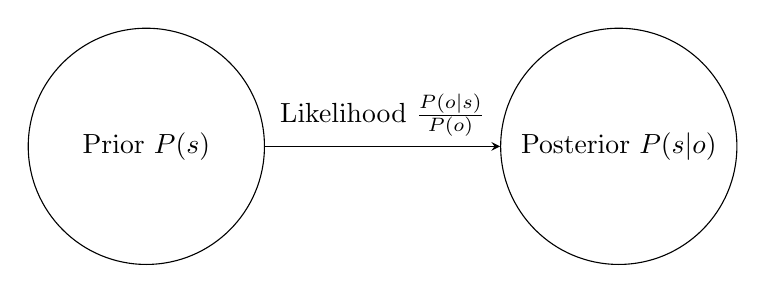
\begin{tikzpicture}[>=stealth, node distance=6cm]
        \node[circle,draw,minimum size=3.0cm] (prior) {Prior $P(s)$};
        \node[circle,draw,minimum size=3.0cm,right of=prior] (posterior) {Posterior $P(s|o)$};
        \draw[->] (prior) -- node[above]{Likelihood $\frac{P(o|s)}{P(o)}$} (posterior);
    \end{tikzpicture}
\end{frame}


\begin{frame}{Perception as Inference}
Suppose we have a model that assigns a probability $P(s)$ to each possible state $s$.
A good model is one that assigns high probability to observations $o$ that are actually encountered, i.e., $P(o|s)$ is high on average when the true state is $s$.
In this view, perception becomes the process of refining internal beliefs to minimize surprise about incoming sensory data.
\end{frame}

\begin{frame}{Information Content and Surprisal}

To enable us to formalize the notion of surprisal, we can think of information content, as introduced by Claude Shannon.

A measure of information content should satisfy three axioms, depending of a probability of an event occuring:
\begin{enumerate}
    \item \textbf{Continuity:} $I$ should vary smoothly with the probabilities.
    \item \textbf{Monotonicity:} If an event becomes less probable, it should carry more information.
    \item \textbf{Additivity:} Independent events should have additive information content.
\end{enumerate}

Under these principles, the information content (or \emph{surprisal}) associated with observing an event $o$ is given by:

\begin{block}{Information content}
    \begin{equation}
        I(o) = -\log P(o)
    \end{equation}
\end{block}

The less likely an event is under our model, the more surprising it is when it occurs.

\end{frame}
\begin{frame}{Expected Surprise and Entropy}

Given a probability distribution $P(s)$ over states $s$, the \emph{expected surprise} quantifies the average amount of surprise we expect to experience upon observing a state drawn from $P$.

The expected surprise is calculated as:

\begin{block}{Entropy}
    \begin{equation}
        \mathbb{E}_{P}[-\   log P(s)] = - \sum_{s} P(s) \log P(s)
    \end{equation}
\end{block}

This quantity is known as the \textbf{entropy} of the distribution $P$.

\vspace{0.3cm}

\begin{itemize}
    \item High entropy $\rightarrow$ High expected surprise $\rightarrow$ Greater uncertainty.
    \item Low entropy $\rightarrow$ Low expected surprise $\rightarrow$ More confident predictions.
\end{itemize}
\end{frame}
\begin{frame}{Visualizing High vs. Low Entropy}

\begin{columns}[T]
    \begin{column}{0.5\textwidth}
        \begin{block}{Low Entropy Distribution}
            \centering
            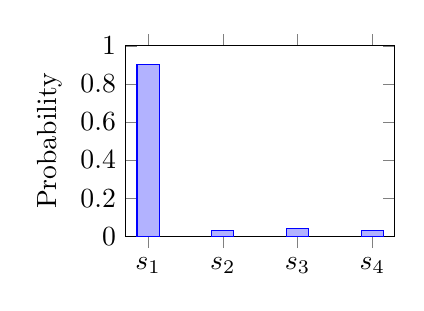
\begin{tikzpicture}
                \begin{axis}[
                    ybar,
                    ymin=0, ymax=1,
                    xtick={1,2,3,4},
                    xticklabels={$s_1$, $s_2$, $s_3$, $s_4$},
                    width=5cm,
                    height=4cm,
                    bar width=8pt,
                    ylabel={Probability}
                ]
                \addplot coordinates {(1,0.9) (2,0.03) (3,0.04) (4,0.03)};
                \end{axis}
            \end{tikzpicture}
            \vspace{0.2cm}
            \begin{itemize}
                \item One dominant state.
                \item Predictable outcome.
            \end{itemize}
        \end{block}
    \end{column}
    
    \begin{column}{0.5\textwidth}
        \begin{block}{High Entropy Distribution}
            \centering
            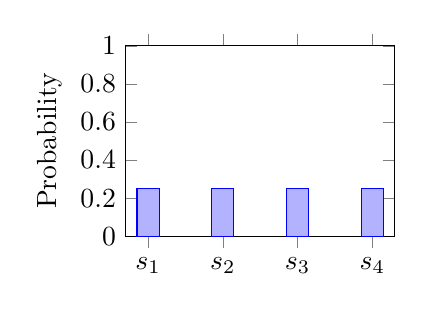
\begin{tikzpicture}
                \begin{axis}[
                    ybar,
                    ymin=0, ymax=1,
                    xtick={1,2,3,4},
                    xticklabels={$s_1$, $s_2$, $s_3$, $s_4$},
                    width=5cm,
                    height=4cm,
                    bar width=8pt,
                    ylabel={Probability}
                ]
                \addplot coordinates {(1,0.25) (2,0.25) (3,0.25) (4,0.25)};
                \end{axis}
            \end{tikzpicture}
            \vspace{0.2cm}
            \begin{itemize}
                \item Many equally likely states.
                \item Uncertain outcome.
            \end{itemize}
        \end{block}
    \end{column}
\end{columns}

\end{frame}
\begin{frame}{Kullback–Leibler (KL) Divergence}
Given two discrete distributions \(P(s)\) (the “true” or “target” distribution) and \(Q(s)\) (an approximate model), the KL–divergence of \(Q\) from \(P\) is
\begin{block}{Definition}
\[
  D_{\mathrm{KL}}\bigl[P \,\|\, Q\bigr]
  \;=\;\sum_{s} P(s)\,\log\frac{P(s)}{Q(s)}
  \;=\;\mathbb{E}_{P}\bigl[\log P(s)-\log Q(s)\bigr].
\]
\end{block}

\begin{itemize}
\item \emph{Relative entropy:} extra surprise (information) when using \(Q\) instead of the true \(P\),
\item \(\;D_{\mathrm{KL}}\ge0\), with equality iff \(P=Q\), 
\item Asymmetric: generally \(D_{\mathrm{KL}}[P\|Q]\neq D_{\mathrm{KL}}[Q\|P]\).
\end{itemize}

\end{frame}
\begin{frame}{Bayesian Surprise: Quantifying Belief Update}
Bayesian surprise measures how much an observation forces us to revise our beliefs.  It is defined as the Kullback–Leibler divergence between posterior and prior distributions.
\begin{block}{Definition}
\[
  \text{Surprise}(o)
  \;=\;D_{\mathrm{KL}}\bigl[P(s\mid o)\,\|\,P(s)\bigr]
  \;=\;\mathbb{E}_{P(\mid o)}\bigl[\log P(s\mid o)-\log P(s)\bigr].
\]
\end{block}

\begin{itemize}
  \item If observation \(o\) does not change our beliefs, \(P(s\mid o)=P(s)\) and surprise is zero.
  \item Large surprise arises when \(P(s\mid o)\) differs substantially from \(P(s)\).
  \item Bayesian surprise captures the \emph{information gain} or \emph{amount of updating} induced by \(o\).
\end{itemize}

\end{frame}

\begin{frame}{Active Inference Agent Summary}
\begin{figure}
    \centering
    \includegraphics[width=0.95\linewidth]{img/model_and_process.png}
    \caption{Active inference agent and environment \footnote{Image source \cite{active-inference-book}}}
    \label{fig:active-inference-agent}
\end{figure}
\end{frame}

\begin{frame}{Limitations of Passive Inference}
Passive inference --- forming beliefs about hidden states based on observations --- is only part of intelligent behavior.  
\medskip

An intelligent agent must also act: influencing its environment to realize preferred outcomes, gather new information, and maintain internal order.

\medskip

Thus, any complete account must unify \textbf{perception} (belief updating) with \textbf{action} (world-changing).
\end{frame}

\begin{frame}{Unifying Perception and Action}
Active inference postulates a single principle for both perception and action:
\begin{itemize}
    \item \textbf{Perception} minimizes surprise by updating beliefs about the world.
    \item \textbf{Action} minimizes surprise by changing the world to align with beliefs.
\end{itemize}

\medskip

Both are understood as minimizing a single quantity: \textbf{expected free energy}, which balances seeking preferred outcomes with reducing uncertainty.
\end{frame}


\section{Variational Inference and Variational Free Energy}
\begin{frame}{Variational Inference and Variational Free Energy}
    \sectionpage
\end{frame}

\begin{frame}{Intractability of Exact Bayesian Inference}
    \begin{block}{Bayes' theorem}
        \begin{equation}
            P(s|o) = \frac{P(o|s)P(s)}{P(o)}
        \end{equation}
        \begin{equation}
            P(o) = \sum_{s}{P(o|s)P(s)}
        \end{equation}
    \end{block}
\end{frame}

\begin{frame}{Problems With Exact Bayesian Inference}
\textbf{Problem:}  
Computing the marginal likelihood \( P(o) \) requires summing over all possible hidden states \( s \).

\medskip

\begin{itemize}
    \item For small or discrete systems, this sum is manageable.
    \item For complex, continuous, or high-dimensional systems, the sum (or integral) becomes \textbf{intractable}.
    \item Exact Bayesian inference becomes computationally prohibitive.
\end{itemize}
\end{frame}

\begin{frame}{Variational Approximation: From Surprise to Free Energy}
\textbf{Key idea:} Replace the true posterior \(P(s\mid o)\) with an approximate distribution \(Q(s)\).  

\medskip

\begin{itemize}
  \item We cannot compute surprise \(-\ln P(o)\) exactly, so instead we derive an \emph{upper bound} on surprise, called the \textbf{variational free energy} \(F[Q,o]\).
  \item Minimizing \(F[Q,o]\) with respect to \(Q\) makes \(Q(s)\) as close as possible to the true posterior.
  \item This procedure is known as \textbf{variational inference}.
\end{itemize}
\end{frame}

\begin{frame}{Upper Bound}
\centering
\includegraphics[width=0.95\linewidth]{img/free_energy_bound.png}  
Surprise upper bound \footnote{Image from \cite{active-inference-book}}
\end{frame}

\begin{frame}{Defining the Surprise Upper Bound}
Assume we have an approximate posterior $Q(s)$ and a true posterior $P(s|o)$. Let us compute their KL-divergence.

\begin{align*}
D_{\mathrm{KL}}[Q(s)\|P(s\mid o)]
&= \sum_{s}Q(s)\log\frac{Q(s)}{P(s\mid o)} \\
&\overset{\text{(Bayes)}}{=} \sum_{s}Q(s)\log\frac{Q(s)\,P(o)}{P(o\mid s)\,P(s)} \\
&= \sum_{s}Q(s)\bigl(\log Q(s) - \log P(s) + \log P(o) - \log P(o\mid s)\bigr) \\
&= \underbrace{\sum_{s}Q(s)\log\frac{Q(s)}{P(s)} - \sum_{s}Q(s)\log P(o\mid s)}_{F[Q,o]}
    \;+
    \underbrace{\sum_{s}Q(s)\log P(o)}_{\log P(o)}
\end{align*}
\end{frame}

\begin{frame}{Surprise bound}
Since KL-divergence is nonnegative, we have found an upper bound of the surprise measure.
\begin{block}{Surprise bound}
    \begin{equation}
        -\log P(o) = -D_{\mathrm{KL}}[Q(s)\|P(s\mid o)] + F[Q,o] \leq F[Q,o]
    \end{equation}
\end{block}

\centering
\includegraphics[width=0.55\linewidth]{img/free_energy_bound.png}  \\
Surprise upper bound \footnote{Image from \cite{active-inference-book}}
\end{frame}

\begin{frame}{Variational Free Energy as an Optimization Objective}
  \begin{block}{Variational free energy}
     \centering
        \begin{align*}
          F[Q,o]
          = \sum_{s}Q(s)\log\frac{Q(s)}{P(s)} \;-\;\sum_{s}Q(s)\log P(o\!\mid\!s) \\
          = D_{\mathrm{KL}}\bigl[Q(s)\,\|\,P(s)\bigr] \;-\;\mathbb{E}_{Q(s)}\bigl[\log P(o\!\mid\!s)\bigr] \\
          = D_{\mathrm{KL}}\bigl[Q(s)\,\|\,P(s\!\mid\!o)\bigr]\;-\;\log P(o)
        \end{align*}
  \end{block}

  \begin{itemize}
    \item Complexity: $D_{\mathrm{KL}}\bigl[Q(s)\,\|\,P(s)\bigr]$  
    \item Accuracy: $\mathbb{E}_{Q(s)}\bigl[\log P(o\!\mid\!s)\bigr]$  
    \item Minimizing \(F\) w.r.t.~\(Q \Rightarrow Q^*(s)\approx P(s\!\mid\!o)\)
    \item Negative free energy (\(-F\)) is connected with another measure commonly used in the context of variational inference, the evidence lower bound (ELBO) on \(\ln P(o)\).
  \end{itemize}
\end{frame}


\section{Expected Free Energy and Action}
\begin{frame}{Expected Free Energy and Action}
    \sectionpage
\end{frame}

\begin{frame}{Beyond Perception: The Need to Act and Plan}
     \begin{block}{Belief-Updating Is Only Half the Story}
    An agent that merely refines its internal model remains a passive observer.  
    Without \emph{planning}, it cannot shape its future—nor test its hypotheses in the real world effectively.
  \end{block}

  \vspace{0.3cm}
  \begin{itemize}
    \item \textbf{Active Sampling:}  
      Actions are the experiments by which an agent tests its model:  
      perception and action form a continuous loop.
    \item \textbf{Temporal Foresight:}  
      Planning lets the agent anticipate downstream consequences,  
      choosing action sequences rather than isolated moves.
    \item \textbf{Goal-Directed Control:}  
      To reach preferred states, the agent must weigh possible futures  
      against its preferences and constraints.
    \item \textbf{Uncertainty Resolution:}  
      By simulating trajectories, the agent can select interventions  
      that promise the greatest reduction in surprise before they occur.
  \end{itemize}
\end{frame}

\begin{frame}{Plans and Policies}
  \begin{block}{From Plans to Policies}
    To formalize planning, we introduce the concept of a \emph{policy} (\(\pi\)):  
    a (possibly conditional) sequence of actions an agent can perform over time.
  \end{block}

  \begin{itemize}
    \item A \textbf{plan} becomes a special case of a policy:  
      a predefined sequence of intended actions without conditional branching.
    \item A \textbf{policy}, more generally, allows for flexibility:  
      actions can depend on intermediate observations.
    \item The agent's fundamental task is to \emph{infer} the most appropriate policy  
      at each time—balancing exploration and exploitation.
  \end{itemize}
\end{frame}

\begin{frame}{An Agent's Task} 
  \begin{block}{Key Question}
    \centering
    \emph{Given my beliefs about the environment, which policy will best minimize my future surprise?}
  \end{block}
\end{frame}

\begin{frame}{Expected Free Energy: Definition}
    Let us define $Q(\tilde{s}, \tilde{o} | \pi)=Q(\tilde{s} | \pi) P(\tilde{o} | \tilde{s})$. Then the expected free energy can be defined in the following way.
    \begin{block}{Expected Free Energy -- EFE}
        \begin{align*}
            G(\pi)=-\underbrace{\mathbb{E}_{Q(\tilde{s}, \tilde{o} | \pi)}[D_{\mathrm{KL}}[Q(\tilde{s}| \tilde{o}, \pi) \| Q(\tilde{s})]]}_{\text{Information gain}} - \underbrace{\mathbb{E}_{Q(\tilde{o}|\pi)}[\ln P(\tilde{o}|C)]}_{\text{Pragmatic value}}
        \end{align*}
    \end{block}

    \begin{itemize}
        \item \textbf{Epistemic value}: favors actions that \emph{reduce uncertainty} about the environment.
        \item \textbf{Pragmatic value}: favors actions that \emph{achieve preferred states} (encoded in \(C\)).
    \end{itemize}
\end{frame}

\begin{frame}{Example: An Organism's Temperature}
    \begin{columns}[T]
        \begin{column}{0.5\textwidth}
            Consider an organism whose survival depends on maintaining its internal temperature within a narrow range.

            \vspace{0.3cm}
        
            On the one hand, it must perform actions that directly ensure its internal temperature remains within this range.  
            On the other hand, it is uncertain which specific policies will best achieve this over time and in changing conditions.
        \end{column}
        \begin{column}{0.5\textwidth}
            \begin{figure}
                \centering
                \includegraphics[width=1.0\linewidth]{img/active_inference_agent.png}
                \caption{Agent mantaining body temperature}
                \label{fig:active-inference-agent}
            \end{figure}
        \end{column}
    \end{columns}
\end{frame}

\begin{frame}{Example: An Organism's Temperature}
    \begin{columns}[T]
        \begin{column}{0.5\textwidth}
            Thus, the organism faces the classic \textbf{explore-exploit dilemma}:  
            it must \emph{exploit} known strategies that are likely to maintain homeostasis, while simultaneously \emph{exploring} to reduce uncertainty about better or more reliable policies.
        
            \vspace{0.4cm}
        
            Both tendencies are unified under the drive to \textbf{minimize expected free energy}.
        \end{column}
        \begin{column}{0.5\textwidth}
            \begin{figure}
                \centering
                \includegraphics[width=1.0\linewidth]{img/active_inference_agent.png}
                \caption{Agent mantaining body temperature}
                \label{fig:active-inference-agent}
            \end{figure}
        \end{column}
    \end{columns}
\end{frame}

\begin{frame}{Epistemic Value: Reducing Uncertainty}
    \begin{block}{Information gain}
        \begin{equation}
            \mathbb{E}_{Q(\tilde{s}, \tilde{o} | \pi)}[D_{\mathrm{KL}}[Q(\tilde{s}| \tilde{o}, \pi) \| Q(\tilde{s})]]
        \end{equation}
    \end{block}

    The first component of the expected free energy rewards policies that are expected to \textbf{reduce uncertainty} about the hidden states of the environment.

    \vspace{0.3cm}

    It measures the \emph{expected information gain}: how much an agent expects to learn by executing a policy.

    \vspace{0.3cm}

    Thus, even actions whose immediate outcomes are uncertain may be valuable, if they are expected to make the world more predictable in the future.

\end{frame}

\begin{frame}{Pragmatic Value: Achieving Outcomes}
    \begin{block}{Pragmatic value}
        \begin{equation}
            \mathbb{E}_{Q(\tilde{o}|\pi)}[\ln P(\tilde{o}|C)]
        \end{equation}
    \end{block}

    The second component of the expected free energy favors policies that are likely to bring about \textbf{preferred outcomes}.

    \vspace{0.3cm}

    Here, \(C\) represents prior preferences over observations:  
    a specification of what states of the world the agent \emph{desires} or \emph{expects} to encounter.

    \vspace{0.3cm}

    In this way, the agent does not merely seek to learn, but actively strives to realize \emph{valued goals}.
\end{frame}

\begin{frame}{Policies as Plans to Minimize EFE}
    \begin{block}{Policy inference}
        Selecting a policy is treated as a problem of inference — the agent infers which policy is most likely to minimize EFE.
    \end{block}
    
    The task solved by an active inference agent, besides refining its generative model of the environment, is the selection of actions over time.
    
    \vspace{0.3cm}
    
    By evaluating and comparing the expected free energy (EFE) of different \emph{policies} — sequences of actions — the agent can estimate their effectiveness and choose the most promising one.
\end{frame}


\section{Building Active Inference Models}
\begin{frame}{Building Active Inference Models}
    \sectionpage
\end{frame}

\begin{frame}{What is a Generative Model?}\textbf{Definition} 
    \begin{block}{Definition}
          A generative model is a \emph{probabilistic} framework that 
          defines a \emph{joint distribution} \(p(x, z)\) over 
          \begin{itemize}
            \item \(x\): observed data,
            \item \(z\): latent (hidden) variables.
          \end{itemize}
    \end{block}
    \begin{itemize}
        \item \emph{Likelihood Evaluation:} Compute \(p(x)\) to assess how probable an observation is:
              \[
                p(x) \;=\;\int p(z)\,p(x\mid z)\,\mathrm{d}z
              \]
        \item \emph{Sampling:} Generate new data by 
              \[
                z\sim p(z),\quad x\sim p(x\mid z).
              \]
        \item Generative: models \(p(x, y)\) or \(p(x, z) \Rightarrow\) can simulate data  
        \item Discriminative: models \(p(y\mid x) \Rightarrow\) only predicts labels
    \end{itemize}
\end{frame}

\begin{frame}{Generative Model Factorization}
  Consider a generative model 
  \[
    p(x_1, x_2, x_3, \dots, x_n).
  \]
  Often, this joint distribution can be decomposed into simpler factors:
  \[
    p(x_1, x_2, \dots, x_n)
      \;=\;\prod_{f=1}^F \phi_f\bigl(x_{f(1)},\,x_{f(2)},\,\dots\bigr),
  \]
  where each factor \(\phi_f\) depends only on a small subset of the variables.  

  \medskip
  
  \begin{itemize}
    \item We will focus on the case, where each factor is a conditional \(P(x_j\!\mid x_k)\).  
    \item  The factorization encodes conditional‐independence: if no factor links \(x_i\) and \(x_j\), then 
      \[
        x_i \;\perp\; x_j 
        \;\bigm|\;
        \text{(the variables they both connect to)}.
      \]
  \end{itemize}
\end{frame}

\begin{frame}{Graphical Models Representation}
    \begin{figure}
        \centering
        \includegraphics[width=0.75\linewidth]{img/graphical_models.png}
        \caption{Graphical models examples \footnote{Image source \cite{active-inference-book}}}
        \label{fig:graphical-model-example}
    \end{figure}
\end{frame}

\begin{frame}{Graphical Models Semantics}
  A factor-graph style graphical model comprises two kinds of nodes and edges that encode dependencies and conditional independencies:
  \begin{itemize}
    \item \textbf{Variable-nodes} (◯)  
      \begin{itemize}
        \item Each represents a random variable \(x_i\).
      \end{itemize}
    \item \textbf{Factor-nodes} ($\Box$)
      \begin{itemize}
        \item Each of them represents a local factor \(\phi_f\bigl(x_{f(1)},\dots\bigr)\), that is a conditional \(P(x_j\mid x_k)\).  
        \item Connects exactly to the variables on which it depends.  
      \end{itemize}
  \end{itemize}
\end{frame}

\begin{frame}{Graphical Models Semantics}
    \begin{itemize}
        \item \textbf{Edges}  
      \begin{itemize}
        \item An edge between a factor and a variable means that the variable appears as an argument of that factor.  
        \item Absence of a path (given conditioning) $\Rightarrow$ conditional independence.
        \item A directed edge into a factor-node indicates the factor is a conditional distribution whose children are the variables on its outgoing edges.
      \end{itemize}
    \item \textbf{Conditional-independence}  
      \[
        x_i \;\perp\; x_j 
        \;\bigm|\;
        \mathcal{S}
        \quad\Longleftrightarrow\quad
        \text{all paths between \(x_i\) and \(x_j\) are goes through }\mathcal{S}.
      \]
    \end{itemize}
\end{frame}

\begin{frame}{Partially Observable Markov Decision Process -- POMDP}
    \begin{figure}
        \centering
        \includegraphics[width=1.0\linewidth]{img/pomd_graphical_model.png}
        \caption{POMDP \footnote{Image source \cite{active-inference-book}}}
        \label{fig:pomd}
    \end{figure}
\end{frame}

\begin{frame}{POMDP in Active Inference}
  \textbf{Dynamic generative model:} Partially-Observable Markov Decision Process (POMDP)
  \[
    p(s_{1:T},o_{1:T},\pi)
      \;=\; p(\pi)\,\prod_{t=1}^T p(s_t \mid s_{t-1},\pi)\,p(o_t\mid s_t)
  \]
  \medskip
  \begin{itemize}
    \item \(\mathbf{s_t}\): hidden state at time \(t\)  
    \item \(\mathbf{o_t}\): observation, depends only on \(s_t\)  
    \item \(\boldsymbol\pi\): policy (sequence of actions), indexes alternative state‐trajectories  
    \item \textbf{Transition model:} \(p(s_t\mid s_{t-1},\pi)\) couples states across time under a chosen policy  
    \item \textbf{Observation model:} \(p(o_t\mid s_t)\) specifies how states generate sensory data  
    \item \textbf{Prior over policies:} \(p(\pi)\) encodes preferences (via expected free energy)  
  \end{itemize}
\end{frame}

\begin{frame}{Inference in POMDP}
    \begin{block}{Policy selection}
        Action selection is just inference over \(\pi\) under one unified generative model.
    \end{block}
\end{frame}

\begin{frame}{Discrete Generative Model for POMDP -- Matrix Formulation}
\[
  P\bigl(\tilde o_{1:T},\,\tilde s_{1:T},\,\pi\bigr)
    \;=\;P(\pi)\;P(s_1\mid\pi)\;\prod_{t=1}^T
       \;P(o_t\mid s_t)\;P\bigl(s_t\mid s_{t-1},\pi\bigr)
\]
\medskip

\begin{description}
  \item[\(A\) – Likelihood]  
    \(A_{o,s} = P(o_t = o\mid s_t = s)\)  
    (how hidden state \(s\) generates observation \(o\))
  \item[\(B^\pi\) – Transitions]  
    \(B^\pi_{s',s} = P(s_t = s'\mid s_{t-1} = s,\;\pi)\)  
    (dynamics under policy \(\pi\))
  \item[\(D\) – Prior over initial state]  
    \(D_{s} = P(s_1 = s)\)
  \item[\(C\) – Prior preferences]  
    \(C_{o}\propto \ln P(o_t = o)\)  
    (encodes which outcomes are “desired”)
  \item[\(P(\pi)\) – Prior over policies]  
    Usually uniform or based on expected free‐energy under each \(\pi\).
\end{description}
\end{frame}

% ——— Slide: Inference & action in discrete POMDP ———
\begin{frame}{Active Inference on a Discrete POMDP}
\textbf{Perception (state‑estimation):}  
Minimize variational free energy \(F\) w.r.t. beliefs \(Q(s_{1:T}\!\mid\!\pi)\):
\[
  Q^*(s_{1:T}\!\mid\!\pi)
  \;=\;\arg\min_{Q}\;F\bigl[Q,\,\tilde o;A,B^\pi,D\bigr]
\]
yields approximate posterior \(Q(s_t)\) as discussed previously.

\medskip
\textbf{Policy selection (planning):}  
Minimize \emph{expected} free energy \(G(\pi)\) under each candidate \(\pi\),
balancing
\[
  \underbrace{\mathbb{E}[\,\underbrace{-\ln P(o\mid s)}_{\text{extrinsic cost}}\,]}_{\text{risk}}
  + 
  \underbrace{\mathbb{E}[\,\underbrace{\ln Q(s\mid\pi) - \ln P(s\mid\pi)}_{\text{information gain}}\,]}_{\text{ambiguity / epistemic value}}
\]
Select  
\(\displaystyle \pi^* = \arg\min_\pi G(\pi)\).

\medskip
\textbf{Action:} execute first action of \(\pi^*\), observe new \(o_{t+1}\), repeat inference.
\end{frame}

\begin{frame}{Linear Algebraic Form of Expected Free Energy (Eq. 4.10)}
\begin{columns}[t]
  \begin{column}{0.4\textwidth}
    \[
    \begin{aligned}
    \pi_0 &= \sigma(-G) \\[6pt]
    G_\pi &= H \, s_{\pi\tau} \;+\; o_{\pi\tau}^\top\,\varsigma_{\pi\tau} \\[4pt]
    \varsigma_{\pi\tau} &= \ln o_{\pi\tau} \;-\; \ln C_\tau \\[4pt]
    H &= -\mathrm{diag}\bigl(A_i \ln A_i\bigr) \\[4pt]
    P(o_\tau \!\mid\! C) &= \mathrm{Cat}(C_\tau) \\[4pt]
    Q(o_\tau \!\mid\! \pi) &= \mathrm{Cat}(o_{\pi\tau}),\quad o_{\pi\tau}=A\,s_{\pi\tau} \\[4pt]
    Q(s_\tau \!\mid\! \pi) &= \mathrm{Cat}(s_{\pi\tau}) \\[4pt]
    Q(s_\tau) &= \mathrm{Cat}(s_\tau),\quad s_\tau = \sum_{\pi} \pi\,s_{\pi\tau}
    \end{aligned}
    \]
  \end{column}
  \begin{column}{0.58\textwidth}
    \begin{itemize}
      \item \(\pi_0\): prior over policies via a softmax of negative expected free energy.  
      \item \(G_\pi\): expected free energy decomposed into “ambiguity” \(H\,s\) and “risk” \(o^\top\varsigma\).  
      \item \(\varsigma\): log–odds of predicted outcomes versus preferred outcomes.  
      \item \(H\): entropy operator on likelihood \(A\).  
      \item \(A\), \(B\), \(C\): likelihood, transition and preference matrices in categorical form.  
      \item \(\mathrm{Cat}(\cdot)\): categorical distribution.  
    \end{itemize}
  \end{column}
\end{columns}
\end{frame}

\begin{frame}{Policy Encoding in Matrix Form}
    \textbf{Policy as transition‐matrix sequence}
    \begin{itemize}
      \item A policy \(\pi\) is a sequence of actions \((a_1,\dots,a_T)\).
      \item Each action \(a_t\) selects a transition matrix \(B^{a_t}\).
      \item Under \(\pi\), the hidden‐state update:
      \[
        s_{\pi\,t}
        = B^{a_t}\,s_{\pi,\,t-1},
        \quad
        B^\pi = B^{a_T}\cdots B^{a_1}.
      \]
      \item Predicted observation:
      \[
        o_{\pi\,t} = A\,s_{\pi\,t}.
      \]
    \end{itemize}
\end{frame}

% ——— Slide: Impact on Expected & Variational Free Energy ———
\begin{frame}{Impact on Free‐Energy Equations}
\begin{columns}[t]
  \begin{column}{0.48\textwidth}
    \textbf{Expected Free Energy (4.10)}  
    \[
      G_\pi
      = \sum_{t=1}^T
        \bigl[H\,s_{\pi\,t}
        + o_{\pi\,t}^\top(\ln o_{\pi\,t}-\ln C_t)\bigr]
    \]
    Policy prior:
    \[
      \pi_0(\pi)=\sigma(-G_\pi)
    \]
  \end{column}
  \begin{column}{0.48\textwidth}
    \textbf{Variational Free Energy (4.11)}  
    \[
      F(\pi)
      = \sum_{t=1}^T
        s_{\pi\,t}^\top\bigl(\ln s_{\pi\,t}
        -\ln A\,o_t
        -\ln B^{a_t}s_{\pi,t-1}\bigr)
    \]
    Note: each \(B^{a_t}\) plugs into the complexity–accuracy trade‐off.
  \end{column}
\end{columns}
\end{frame}

\begin{frame}{Variational Free Energy under a Policy (Eq. 4.11)}
\[
\begin{aligned}
F(\pi) &= \sum_{\tau} F_{\pi\tau}, \\[4pt]
F_{\pi\tau}
&= 
s_{\pi\tau}^\top
\Bigl(\ln s_{\pi\tau} - \ln A\,o_\tau - \ln B_\pi\,s_{\pi,\tau-1}\Bigr)
\end{aligned}
\tag{4.11}
\]
\begin{itemize}
  \item \(F(\pi)\) is the variational free energy for policy \(\pi\), summing over all time steps.  
  \item Each term \(F_{\pi\tau}\) combines “complexity” (\(\ln s\)) and “accuracy” (\(\ln A\,o\), \(\ln B\,s\)).  
  \item Minimizing \(F(\pi)\) drives inference about the hidden‐state trajectories under \(\pi\).  
\end{itemize}
\end{frame}

\begin{frame}{Inference of Hidden‐State Beliefs}
    \textbf{Gradient‐based update}
    \[
      s_{\pi\tau} \;=\;\sigma\bigl(v_{\pi\tau}\bigr), 
      \qquad
      \dot v_{\pi\tau}
      = -\,\nabla_{s_{\pi\tau}}\,F_{\pi\tau}
    \]
    \[
      \nabla_{s_{\pi\tau}}F_{\pi\tau}
      = \ln s_{\pi\tau}
        - \ln A\,o_{\tau}
        - \ln B^{\pi}\,s_{\pi,\tau-1}
        - \ln B^{\pi+1\,\top}\,s_{\pi,\tau+1}
    \]
    \begin{itemize}
      \item Interpret \(v\) as log‑odds; gradient flow drives \(F\downarrow\).  
      \item Softmax \(\sigma\) ensures \(\sum s_{\pi\tau}=1\).  
      \item Analogy: like backprop in NN, but on free‑energy landscape.  
    \end{itemize}
\end{frame}

% ——— Slide 2: Policy‐belief inference via softmax gradient ———
\begin{frame}{Inference of Policy Beliefs}
    \textbf{Gradient condition for optimal policy}
    \[
      \nabla_{\pi}F = 0
      \;\Longrightarrow\;
      \pi 
      = \sigma\bigl(-\,G \;-\; F\bigr)
    \]
    \begin{itemize}
      \item \(G\): expected free energy (future‑directed cost).
      \item \(F\): variational free energy (past/present fit). 
    \end{itemize}
    \centering
    \vspace{1em}
    \begin{tikzpicture}[scale=0.8]
      \node[draw, circle] (G) at (0,1) {\(-G\)};
      \node[draw, circle] (F) at (0,-1) {\(-F\)};
      \node[draw, rectangle] (sum) at (2,0) {\(-G - F\)};
      \node[draw, circle, right=of sum] (pi) {\(\pi\)};
      \draw[->] (G) -- (sum);
      \draw[->] (F) -- (sum);
      \draw[->] (sum) -- (pi) node[midway,above]{\(\sigma\)};
    \end{tikzpicture}
\end{frame}

\section{Conclusion and Outlook}
\begin{frame}{Conclusion and Outlook}
    \sectionpage
\end{frame}

\begin{frame}{Recap: Core Ideas}
    
\end{frame}

\begin{frame}{What Active Inference Explains}
\end{frame}

\begin{frame}{Future Directions and Open Questions}
\end{frame}

\begin{frame}{Questions and Discussion}
\end{frame}

\begin{frame}{Bibliography}
\bibliography{bibliography}{}
\bibliographystyle{plain}
\end{frame}

\end{document}